\chapter{Model liniowy obiektu i regulacja}
\label{cha:ch6_model_liniowy}

Do wyznaczenia regulatorów dla systemu konieczne jest uzyskanie jego uproszczonego modelu liniowego, który --- w myśl twierdzenia Hartmana-Grobmana --- zachowuje się podobnie jak obiekt nieliniowy. Zgodnie z teorią sterowania, wyznaczone w tym rozdziale regulatory powinny działać w odchyłkach wybranego punktu pracy.

%%%%
\section{Punkt pracy i linearyzacja}
\label{sec:ch6_punkt_pracy_linearyzacja}

Za zmienne stanu przyjęto: położenie liniowe kulki względem środka belki $x_1$, kąt obrotu belki względem poziomu $x_3$ oraz ich pochodne w czasie $x_2 = \dot{x_1}$, $x_4 = \dot{x_3}$.

\begin{figure}[h]
    \centering
    \includesvg[width=0.5\textwidth,svgpath=./vector_graphics/]{zmienne_stanu}
    \caption{Reprezentacja głównych zmiennych stanu w obiekcie.}
    \label{fig:zmienne_stanu}
\end{figure}

Jak naturalny wybrano punkt pracy $x^*$, w którym wszystkie zmienne stanu są zerowe:
\begin{equation}
    x^* = \begin{bmatrix}
    0 \\
    0 \\
    0 \\
    0 \\
    \end{bmatrix}
\end{equation}

Linearyzację modelu przeprowadzono z wykorzystaniem narzędzi wbudowanych w pakiet \textsc{Mat\-lab/Si\-mu\-link}, a konkretnie \texttt{Linear Analysis Tool}. Do linearyzacji przygotowano wersję mo\-de\-lu układu z odłączonym wejściem na zakłócenia oraz wyłączoną (za pomocą bloku \textit{Manual Switch}) częścią odpowiedzialną za symulację tarcia suchego w silniku (\cref{fig:sm_linearization}). Usunięcie tarcia suchego w~przypadku linearyzacji w punkcie równowagi $x^*$ spowodowane jest względami praktycznymi: częsta zmiana znaku prędkości obrotowej belki utrudnia lub nawet uniemożliwia uruchamianie symulacji, gdyż wewnętrzny mechanizm \textsc{Simulink} wykrywa wtedy wiele przejść przez zero\footnote{Możliwe jest wyłączenie tego mechanizmu lub użycie metody adaptacyjnej wykrywania przejść przez zero, jednakże spowalnia to symulację.}.

\begin{figure}[h]
    \centering
    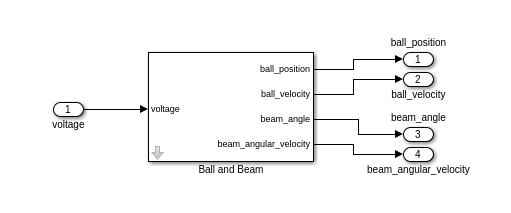
\includegraphics[width=0.9\textwidth]{sm_linearization}
    \caption{Model układu przeznaczony do przeprowadzenia linearyzacji.}
    \label{fig:sm_linearization}
\end{figure}

Przed linearyzacją konieczne było znalezienie punktu pracy, czyli przeprowadzenie tzw. \textit{trimmingu} modelu. W procesie tym wyznacza się ograniczenia na stany układu lub ich wartości początkowe. Jest to istotne zagadnienie, gdyż układ zbudowany za pomocą przybornika \textsc{Simscape Multibody} zawiera \num{18} stanów, chociaż, tak jak to zdefiniowano na początku rozdziału, wybrano jedynie \num{4} do prezentacji systemu. Większość z tych ,,nadmiarowych'' stanów to położenia i prędkości złącz pryzmatycznych lub obrotowych, które nie są istotne z punktu widzenia reprezentacji liniowej układu.

\textit{Trimming} modelu to tak naprawdę proces optymalizacyjny, mający na celu tak dobrać wartości początkowe stanów systemu, aby maksymalny ich błąd w trakcie symulacji był jak najmniejszy; jest to jednoznaczne z numerycznym znajdowaniem punktu równowagi systemu. Z powodu swojej optymalizacyjnej natury, proces ten nie mógł znaleźć odpowiedniego punktu, dopóki nie został rozpoczęty z odpowiednio bliskiego otoczenia punktu równowagi. Osiągnięto to podając jako wartość startową dla wejścia bloku (\textit{voltage} na \cref{fig:sm_linearization}) napięcie sterowania $u = -0,51158$. Wartość ta wynika z faktu delikatnego ciążenia belki w stronę mechanizmu korbowego, co musi rekompensować silnik poprzez wytworzenie niezerowego momentu.

Po wyznaczeniu punktu równowagi, nadal wykorzystując narzędzie \texttt{Linear Analysis Tool}, zlinearyzowano układ otrzymując wynikowe macierze:

\begin{align}
    \widetilde{A} &= \begin{bmatrix}
        0 & 1 & 0 & 0 \\
        -0,2289 & 0 & 47,607 & 3,2117 \\
        0 & 0 & 0 & 1 \\
        0,4977 & 0 & 0,262 & -6,9832 \\
    \end{bmatrix} \nonumber \\
    \widetilde{B} &= \begin{bmatrix}
        0 \\
        -15,5016 \\
        0 \\
        33,7051 \\
    \end{bmatrix} \nonumber \\
    \widetilde{C} &= \begin{bmatrix}
            0,03 & 0 & 0 & 0 \\
            0 & 0,03 & 0 & 0 \\
            0 & 0 & 0,2044 & 0 \\
            0 & 0 & 0 & 0,2044 \\
    \end{bmatrix} \nonumber \\
    \widetilde{D} &= 0 \label{eq:macierze_stanu1}
\end{align}

Dalsza analiza wyników linearyzacji wykazała, że narzędzie \texttt{Linear Analysis Tool} dobrało inne zmienne stanu niż oczekiwane, a mianowicie:

\begin{itemize}
    \item $\tilde{x}_1$ -- kąt obrotu kulki wokół własnej osi,
    \item $\tilde{x}_2$ -- prędkość kątowa obrotu kulki wokół własnej osi,
    \item $\tilde{x}_3$ -- kąt obrotu wału motoreduktora,
    \item $\tilde{x}_4$ -- prędkość kątowa obrotu wału motoreduktora.
\end{itemize}

Należy zauważyć, że kąt obrotu kulki wokół własnej osi $\tilde{x}_1$ oraz przesunięcie liniowe kulki $x_1$ są ze sobą liniowo zależne: $\tilde{x}_1 = r x_1$, gdzie $r$ to promień kulki. Podobnie kąty obrotu belki $x_3$ i obrotu wału motoreduktora $\tilde{x}_3$ również są od siebie liniowo zależne w pobliżu punktu pracy, co zostało wskazane w rozdziale \ref{sec:ch3_uklad_napedowy}, wzór \eqref{eq:uproszczona_zaleznosc_kata_belki}. Oznacza to, że można dokonać transformacji macierzy stanu \eqref{eq:macierze_stanu1} tak, aby otrzymać oczekiwane zmienne stanu.

Transformację podobieństwa zmiennych stanu $\breve{x} = T_1 \tilde{x}$ przeprowadza się następująco:
\begin{align}
    \breve{x}' &= T_1 \widetilde{A} T_1^{-1} \breve{x} + T_1 \widetilde{B} u \nonumber \\
    \breve{y} &= \widetilde{C} T_1^{-1} \breve{x} + \widetilde{D} u \label{eq:transformacja_x}
\end{align}

Jako macierz transformacji $T_1$ użyto macierzy wyjścia $\widetilde{C}$ i otrzymano następujące macierze wynikowe:
\begin{align}
    \breve{A} &= \begin{bmatrix}
         0 & 1 & 0 & 0 \\
         -0,2289 & 0 & 6,9871 & 0,4714 \\
         0 & 0 & 0 & 1 \\
         3,3914 & 0 & 0,262 & -6,9832 \\
    \end{bmatrix} \nonumber \\
    \breve{B} &= \begin{bmatrix}
         0 \\
         -0,465 \\
         0 \\
         6,8896 \\
    \end{bmatrix} \nonumber \\
    \breve{C} &= \begin{bmatrix}
        1 & 0 & 0 & 0 \\
        0 & 1 & 0 & 0 \\
        0 & 0 & 1 & 0 \\
        0 & 0 & 0 & 1 \\
    \end{bmatrix} \nonumber \\
    \breve{D} &= 0 \label{eq:macierze_stanu2}
\end{align}

% TODO: lepsza argumentacja?
Jak można zaobserwować, położenie zer i jedynek w macierzach $\widetilde{A}$ i $\breve{A}$ pozostało takie samo, co potwierdza, że dokonana została transformacja liniowa.

%%%%
\section{Kaskadowy układ regulacji}
\label{sec:ch6_kaskadowy_uklad_regulacji}

Należy zauważyć, że belka wraz z mechanizmem napędowym tworzą szybki, nieliniowy, niejednoznaczny i łatwo zakłócany układ, podczas gdy kulka jest obiektem wolnym, liniowym i stacjonarnym. Ta ,,rozdzielność'' dwóch układów sugeruje możliwość zastosowania dwóch regulatorów.

Ponadto w tym obiekcie regulacji zastosowano silnik prądu stałego zamiast rozwiązania z wbudowanym regulatorem pozycji, na przykład serwonapędem modelarskim (porównanie alternatywnych do zastosowanego wariantów zespołu napędowego umieszczono w dodatku \ref{appA_warianty_zespolu_napedowego}). W wyniku dzia\-łania tego silnika następuje ruch belki, który powoduje ruch kulki. Masa kulki jest niewielka, a zatem nie wpływa praktycznie wcale na ruch belki.

% TODO: czas teraźniejszy?!
Korzystając z powyższych obserwacji i wspomnianego ciągu następstw, w niniejszej pracy proponuje się zastosowanie kaskadowego układu regulacji, w którym regulator nadrzędny pozycji kulki generuje sygnał sterujący dla regulatora podrzędnego wychylenia belki. Schemat ilustrujący taką strukturę sterowania przedstawiony jest na \cref{fig:kaskadowy_uklad_regulacji}.

\begin{figure}[h]
    \centering
    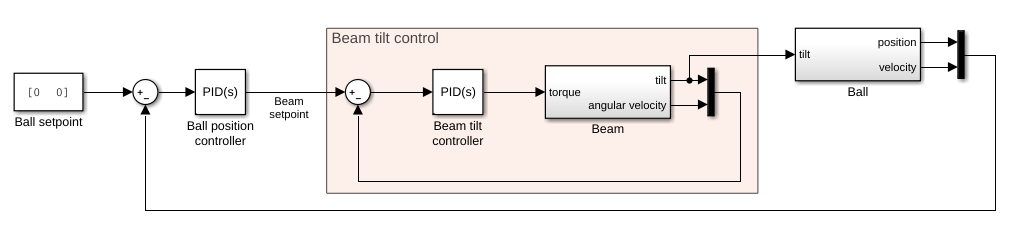
\includegraphics[width=1\textwidth]{kaskadowy_uklad_regulacji}
    \caption{Schemat ilustrujący ideę kaskadowego układu regulacji obiektu typu kulka i~belka.}
    \label{fig:kaskadowy_uklad_regulacji}
\end{figure}

\pagebreak

Aby możliwe było obliczenie osobnych regulatorów dla kulki oraz dla belki, równanie stanu powinno mieć następującą strukturę:

\begin{equation}
    \renewcommand\arraystretch{2}
    \begin{matrix}
        \text{kulka}~\Bigg\{ \\
        \text{belka}~\Bigg\{ 
    \end{matrix}
    \renewcommand\arraystretch{1}
    \left[
    \begin{array}{c}
        \bar{x}_1' \\
        \bar{x}_2' \\
        \hline
        \bar{x}_3' \\
        \bar{x}_4'
    \end{array}
    \right]
    =
    \underbrace{
        \renewcommand\arraystretch{2}
        \left[
        \begin{array}{c|c}
           \bar{A}_{11} & \bar{A}_{12} \\
           \hline
           0 & \bar{A}_{22}
        \end{array}
        \right]
    }_{\bar{A}}
    \left[
    \begin{array}{c}
        \bar{x}_1 \\
        \bar{x}_2 \\
        \hline
        \bar{x}_3 \\
        \bar{x}_4 \\
    \end{array}
    \right]
    +
    \underbrace{
        \renewcommand\arraystretch{2}
        \left[
        \begin{array}{c}
        0 \\
        \hline
        \bar{B}_2
        \end{array}
        \right]
    }_{\bar{B}}
    u \label{eq:warunki_kaskady}
\end{equation}

Z \eqref{eq:warunki_kaskady} wynika, że zachowanie kulki zależy od kulki i belki, a nie zależy od sterowania, natomiast zachowanie belki zależy tylko od belki i sterowania:

\begin{align*}
    \begin{bmatrix}
        \bar{x}_1' \\ \bar{x}_2'
    \end{bmatrix}
    &= \begin{bmatrix}
    \bar{A}_{11} & \bar{A}_{12}
    \end{bmatrix} \bar{x} \\
    \begin{bmatrix}
    \bar{x}_3' \\ \bar{x}_4'
    \end{bmatrix}
    &= \begin{bmatrix}
    0 & \bar{A}_{22}
    \end{bmatrix} \bar{x}
    + \bar{B}_2 u
\end{align*}

Jak można łatwo zauważyć, struktury macierzy $\breve{A}$ i $\breve{B}$ \eqref{eq:macierze_stanu2} nie odpowiadają strukturom pożądanych macierzy $\bar{A}$ i $\bar{B}$. Może to być spowodowane bezwładnością kulki: w momencie ruchu belki w dół, kulka pod wpływem tarcia przesuwa się odrobinę względem powierzchni belki w stronę przeciwną do kierunku spadku (ilustracja na \cref{fig:przeciwny_ruch_kulki}). Sugeruje to niewielka i ujemna zależność przyspieszenia kątowego kulki $\breve{x}_2'$ od sterowania~$u$, podczas gdy zależność belki od sterowania ma znak dodatni i dużo większy współczynnik.

\begin{figure}[h]
    \centering
    \includesvg[width=0.6\textwidth,svgpath=./vector_graphics/]{przeciwny_ruch_kulki}
    \caption{Ilustracja toczenia się kulki w przeciwną stroną niż kierunek spadku.}
    \label{fig:przeciwny_ruch_kulki}
\end{figure}

Kompensacji takiego ruchu kulki, a więc doprowadzenia macierzy $\breve{B}$ do struktury macierzy $\bar{B}$, można dokonać przez transformację $\hat{x} = T_2 \breve{x}$ zdefiniowaną jak w \eqref{eq:transformacja_x}; za macierz $T_2$ dobrano:
\begin{equation}\label{eq:transformacja2_x}
    \renewcommand\arraystretch{1.2}
    T_2 = \begin{bmatrix}
        1 & 0 & -\frac{\breve{B}_2}{\breve{B}_4} & 0 \\
        0 & 1 & 0 & -\frac{\breve{B}_2}{\breve{B}_4} \\
        0 & 0 & 1 & 0 \\
        0 & 0 & 0 & 1 \\
    \end{bmatrix}
\end{equation}
gdzie $\breve{B}_i$ oznacza \textit{i}-ty element macierzy $\breve{B}$.
% TODO: skąd się bierze ten współczynnik?!?!?!?!

Dzięki przekształceniu przez macierz \eqref{eq:transformacja2_x} otrzymano następujące macierze stanu:
\begin{align}
    \hat{A} &= \begin{bmatrix}
    0 & 1 & 0 & 0 \\
    0 & 0 & 7,0047 & 0 \\
    0 & 0 & 0 & 1 \\
    3,3914 & 0 & 0,0331 & -6,9832 \\
    \end{bmatrix}
    =
    \renewcommand\arraystretch{2}
    \left[
        \begin{array}{c|c}
        \hat{A}_{11} & \hat{A}_{12} \\
        \hline
        \hat{A}_{21} & \hat{A}_{22}
        \end{array}
    \right] \nonumber \\
    \hat{B} &= \begin{bmatrix}
    0 \\
    0 \\
    0 \\
    6,8896 \\
    \end{bmatrix} \nonumber \\
    \hat{C} &= \begin{bmatrix}
    1 & 0 & -0,0675 & 0 \\
    0 & 1 & 0 & -0,0675 \\
    0 & 0 & 1 & 0 \\
    0 & 0 & 0 & 1 \\
    \end{bmatrix} \nonumber \\
    \hat{D} &= 0 \label{eq:macierze_stanu3}
\end{align}

Widać, że postać macierzy $\hat{B}$ z \eqref{eq:macierze_stanu3} odpowiada już oczekiwanej strukturze, natomiast macierz $\hat{A}$~jeszcze nie ma takiej formy. W związku z tym zdecydowano się doprowadzić macierz $\hat{A}$ do postaci blokowo-trójkątnej górnej poprzez wyzerowanie $\hat{A}_{21}$. Nowe macierze stanu przedstawiają się następująco:
\begin{align}
    A &= \begin{bmatrix}
    0 & 1 & 0 & 0 \\
    0 & 0 & 7,0047 & 0 \\
    0 & 0 & 0 & 1 \\
    0 & 0 & 0,0331 & -6,9832 \\
    \end{bmatrix} \nonumber \\
    B &= \begin{bmatrix}
    0 \\
    0 \\
    0 \\
    6,8896 \\
    \end{bmatrix} \nonumber \\
    C &= \begin{bmatrix}
    1 & 0 & -0,0675 & 0 \\
    0 & 1 & 0 & -0,0675 \\
    0 & 0 & 1 & 0 \\
    0 & 0 & 0 & 1 \\
    \end{bmatrix} \nonumber \\
    D &= 0 \label{eq:macierze_stanu4}
\end{align}

Aby udowodnić, że wyzerowanie ww. elementu macierzy $\hat{A}$ nie przyniosło negatywnych skutków, poniżej przedstawiono wykresy charakterystyk amplitudowo-fazowych dla systemów opisanych macierzami $\hat{A}$, $\hat{B}$, $\hat{C}$ i $\hat{D}$ oraz $A$, $B$, $C$ i $D$.

Jak widać na \cref{fig:charakterystyka_amplitudowo_fazowa}, w bardzo niskich częstotliwościach (poniżej \SI{1}{\hertz}) układy nie zachowują się jednakowo. Wynika to z faktu, że przy tak powolnych ruchach belką kulka jest w stanie potoczyć się dalej od środka belki, a zatem jej oddziaływanie na belkę rośnie. Jednakże w wyższych częstotliwościach charakterystyki układów są takie same i w związku z tym można założyć, że macierze wynikowe $A$, $B$, $C$ i $D$ są poprawne.

Ostatecznie uzyskano następujące równania stanu:
\begin{align}
\begin{bmatrix}
    \dot{x}_1 \\ \dot{x}_2 \\ \dot{x}_3 \\ \dot{x}_4
\end{bmatrix}
&= \begin{bmatrix}
    0 & 1 & 0 & 0 \\
    0 & 0 & 7,0047 & 0 \\
    0 & 0 & 0 & 1 \\
    0 & 0 & 0,0331 & -6,9832
\end{bmatrix}
\begin{bmatrix}
    x_1 \\ x_2 \\ x_3 \\ x_4
\end{bmatrix}
+
\begin{bmatrix}
    0 \\ 0 \\ 0 \\ 6,8896
\end{bmatrix}
u \label{eq:rownania_stanu} \\%\displaybreak\\
\begin{bmatrix}
    y_1 \\ y_2 \\ y_3 \\ y_4
\end{bmatrix}
&= \begin{bmatrix}
    1 & 0 & -0,0675 & 0 \\
    0 & 1 & 0 & -0,0675 \\
    0 & 0 & 1 & 0 \\
    0 & 0 & 0 & 1 \\
\end{bmatrix}
\begin{bmatrix}
x_1 \\ x_2 \\ x_3 \\ x_4
\end{bmatrix} \label{eq:rownania_wyjscia} 
\end{align}

\begin{figure}[h]
    \centering
    \includesvg[width=1\textwidth,svgpath=./vector_graphics/]{ch_amplitudowo_fazowa}
    \caption{Wykresy amplitudowo-fazowe systemów opisanych macierzami \eqref{eq:macierze_stanu3} oraz \eqref{eq:macierze_stanu4}. Przedstawiona charakterystyka dla pierwszej zmiennej stanu (położenia linio\-wego kulki).}
    \label{fig:charakterystyka_amplitudowo_fazowa}
\end{figure}

%%%%
\section{Regulator pochylenia belki}
\label{sec:ch6_regulator_belki}

Jako regulator pochylenia belki wybrano prosty regulator proporcjonalny od stanu. Struktura regulacji przedstawiona jest na 

\begin{figure}[ht]
    \centering
    
    \begin{tikzpicture}[auto, node distance=1cm,>=latex']
        \node [input, name=input] {};
        \node [sum, right=of input] (sum) {};
        \node [gain, right=of sum] (controller) {$K$};
        \node [block, right=of controller] (plant) {$G(s)$};
        \node [output, right=of plant] (output) {};
        \draw [draw,->] (input) -- node {$U(s)$} (sum);
        \draw [->] (sum) -- node {} (controller);
        \draw [->] (controller) -- node {} (plant);
        \draw [->] (plant) -- node [name=y] {$Y(s)$}(output);
        \draw [->] (y) -- ++ (0,-2) -| node [pos=0.99] {$-$} (sum);
    \end{tikzpicture}
    
    \caption{Schemat regulacji liniowego systemu regulacji pochyleniem belki.}
    \label{fig:schemat_regulacji_belka}
\end{figure}



% TODO: regulator od stanu

%%%%
\section{Regulator pozycji kulki}
\label{sec:ch6_regulator_kulki}

% TODO: regulator od stanu

%%%%
\section{Podsumowanie}

% TODO: dokończ

%---------------------------------------------------------------------------